\documentclass[10pt]{beamer}

\usetheme{metropolis}
\usepackage{appendixnumberbeamer}

\usepackage{booktabs}
\usepackage[scale=2]{ccicons}

\usepackage{pgfplots}
\usepgfplotslibrary{dateplot}

\usepackage{xspace}

\usepackage{tikz}
    \usetikzlibrary{positioning}

%\usepackage{listings}
\usepackage{minted}

\usepackage{bm}%................................. Bold math symbols (after fonts)

\setbeamercolor{normal text}{bg=white}





\title{EML4930/EML6934: Lecture 00 - About Python }
\subtitle{Python2 vs Python3, Hello World, IPython, Notebooks, Installation}
\date{August 24, 2017}
%\author{CJ}
\author{Charles Jekel}
%\titlegraphic{\includegraphics{images/avatarCropped.png}\vspace{58cm}}
%\institute{1. University of Florida\\ 2. Stellenbosch University, South Africa}

% \titlegraphic{\hfill\includegraphics[height=1.5cm]{logo.pdf}}

\begin{document}

\maketitle

\begin{frame}{About me}
PhD Student in the MDO lab. 

I look at improving techniques for selecting material parameters.

My interests:
\begin{itemize}
\item non-linear finite element (FE) method
\item non-linear material modeling
\item inverse analysis
\item optimization
\item regression and classification
\item digital image correlation (DIC)
\item high performance computing (HPC)
\item Python
\end{itemize}

For more see \url{http://jekel.me}

\end{frame}

\begin{frame}{About the course}
Syllabus available online.

The intention of this course is to prepare you to for doing numerical work in Python.

Course expectations:
\begin{itemize}
\item 12 out of 14 homework | 60~\%
\item 2 quizzes | 10~\%
\item 1 final exam | 30~\%
\end{itemize}


\end{frame}

\begin{frame}{Intended audience}
	\begin{alertblock}{Course description}
Python is a general purpose programming language. Course covers the basics, linear algebra, plotting, and more to prepare students for solving numerical problems. Prerequisite: COP 2271 MATLAB or equivalent.
	\end{alertblock}

\textbf{You already know how to program in some language. \\
You are interested in doing numerical analysis in Python.} 
\end{frame}

\begin{frame}{What is Python? - python.org}
Let's see what \url{http://python.org} has to say about Python.
      	
      	\begin{figure} 	
 	
\includegraphics[width=0.65\textwidth]{figs/pythonLogo.png}
      \end{figure}

\textbf{Python is}
\begin{itemize}
\item an interpreted, object-oriented, high-level programming language with dynamic semantics
\item very attractive for Rapid Application Development
\item a simple and easy to learn syntax
\end{itemize}
\end{frame}

\begin{frame}{Python is a very popular programming language}
For the first time ever, IEEE Spectrum rated Python the most popular programming language in 2017. \url{http://spectrum.ieee.org/computing/software/the-2017-top-programming-languages}
\begin{figure}
 	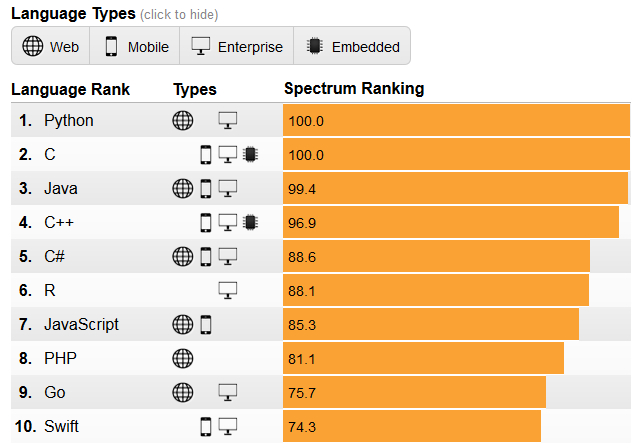
\includegraphics[width=0.85\textwidth]{figs/ieee.png}
\end{figure}
\end{frame}

\begin{frame}{Built using Python}
\begin{figure}
\includegraphics[width=1.0\textwidth]{figs/logos.png}
\end{figure}
\end{frame}

\begin{frame}{Why Python? - Free, Open, and Powerful}
  \begin{columns}[onlytextwidth]
    \column{0.7\textwidth}
\begin{itemize}
\item Python is Free and Open
\item Python can be used commercially 
\item From research to deployment
\item Libraries to do everything
\item Adapted by scientist and engineers
\item Cross platform support
\end{itemize}
    \column{0.3\textwidth}
          \begin{figure} 	
 	
\includegraphics[width=1.0\textwidth]{figs/free-beer.jpg}
      \end{figure}
  \end{columns}
\end{frame}

\begin{frame}{Python2 vs Python3}
There is a syntax difference between Python version 2 and Python version 3. 

When Python 3.0 was released in 2008 it broke backwards compatibility with Python 2.X. This was a mistake, and resulted in a very slow adaption of Python 3. 

There are likely Python libraries that have yet to be ported to Python3. 

Additionally there are libraries that were only written in Python3. 

All new code should probably be written in a Python3 syntax, but I won't force you to use Python3. I still primarily use Python~2.7. Choose your version based on your library needs.

For more see: \url{https://wiki.python.org/moin/Python2orPython3}
\end{frame}

\begin{frame}{Python2 vs Python3 comparison}
  \begin{columns}[onlytextwidth]
    \column{0.5\textwidth}
\textbf{Python2 wins}
\begin{itemize}
\item Speed - Python 2.7 will always be faster
\item Legacy
\item Python updates won't break your code!
\end{itemize}
    \column{0.5\textwidth}
\textbf{Python3 wins}
\begin{itemize}
\item Unicode identifiers
\item Strings unicode by default
\item Simple matrix multiplication with @
\end{itemize}
  \end{columns}
\end{frame}

\begin{frame}{TensorFlow and Windows - you need Python 3.5}
\begin{figure}

\includegraphics[width=0.5\textwidth]{figs/tf.png}
\end{figure}
If you are intested in using \textbf{TensorFlow on Windows,} you must use a very specific version of Python. 

TensorFlow is a state-of-the-art machine learning library. 

See \url{https://www.tensorflow.org/install/install_windows}
\end{frame}

\begin{frame}{Ways to run Python}
Here is the Python2 hello world program saved as helloWorld2.py
\inputminted{python}{code/helloWorld2.py}


These are some of the ways to run Python.
\begin{itemize}
\item from an IDE (integrated development environment)
\item python
\item python helloWorld2.py
\item ipython
\item (while in IPython) \%run helloWorld2.py
\item ipython qtconsole (qtconsole has added benefits)
\item ipython notebook
\end{itemize}
\end{frame}

\begin{frame}{python3 helloWorld2.py}
Running this (helloWorld2.py) in Python3:
\inputminted{python}{code/helloWorld2.py}
gives me the following error:
\begin{figure} 	
 	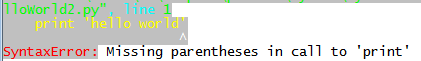
\includegraphics[width=1.0\textwidth]{figs/print23.png}
\end{figure}
because in Python3 \textit{print} is now a function
\end{frame}

\begin{frame}{python3 helloWorld3.py}
With Python 3.X \textit{print} must include an open and closed parentheses. 

The following code is saved as helloWorld3.py
\inputminted{python}{code/helloWorld3.py}

You can run this code with both python2 and python3.
\end{frame}

\begin{frame}{If you want to write code for Python 2.7 and Python 3.X}
Your *.py script should always begin with these first three lines. The following code was saved as helloWorld.py.
\inputminted{python}{code/helloWorld.py}
This code runs with both python2 and python3. 
\end{frame}

\begin{frame}{Using future will force you to write in the Python 3.X syntax}
Executing the following in python2
\inputminted{python}{code/helloWorldBroke.py}
Will give you an error!
\end{frame}

\begin{frame}{Python 3.X allows you to use unicode identifiers}
\'{e} is a unicode character which can be used in the identifier (as a variable) in Python~3.X but not Python~2.X.

Additionally strings in Python~3.X default to unicode (not the case in Python~2.X).

The following code will only run in python3 (unicode breaks my syntax highlighting...)

Fr\'{e}chet = 'Fr\'{e}chet is famous a French mathematician'

print(Fr\'{e}chet)

\end{frame}

\begin{frame}{Comparing strings to numbers in Python 2 is weird}
The following is input and output with python2 (it is not suppose to make any sense). 
\mint{python}|'123' > 900|
True
\mint{python}|'123' > 0|
True
\mint{python}|'123' < 900|
False
\mint{python}|'123' < 0|
False

\textbf{Do not compare different data types in Python 2.X!}
\end{frame}

\begin{frame}{Python 3.X fixes string to number comparison}
by not letting you compare data types that don't make sense
\begin{figure}
 	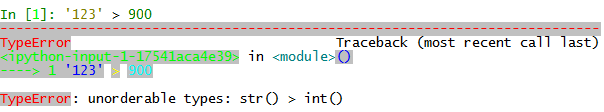
\includegraphics[width=1.0\textwidth]{figs/stringToIntPython3.png}
\end{figure}
\end{frame}

\begin{frame}{Python 2.7 vs Python 3.X depends on you}
Syntax differences:
\begin{itemize}
\item Python 3.X requires print to use parentheses
\item In Python 3.X print is a function
\item You can access the print function of Python~3.X in Python~2.7 by importing \textit{Future print function}
\end{itemize}


Additional resources:
\begin{itemize}
\item \url{http://python-future.org/imports.html}
\item \url{https://wiki.python.org/moin/Python2orPython3}
\item \url{https://learntocodewith.me/programming/python/python-2-vs-python-3/}
\end{itemize}

No more time for Python 2.7 vs Python 3.X. Pick one. Everything we do in this course will be compatible in both versions. You're allowed to use the version that best suits you. 
\end{frame}

\begin{frame}{Install python - do not install from \url{https://python.org}}
Python builds from \url{https://www.python.org/downloads/} do not include pre-built libraries for numerical and scientific work. Compiling and building libraries is very complicated on Windows (and slightly less complicated on other operating systems). Think of this download as the bare basic Python with no libraries.

\textbf{DO NOT DOWNLOAD, DO NOT INSTALL.}
\begin{figure}
 	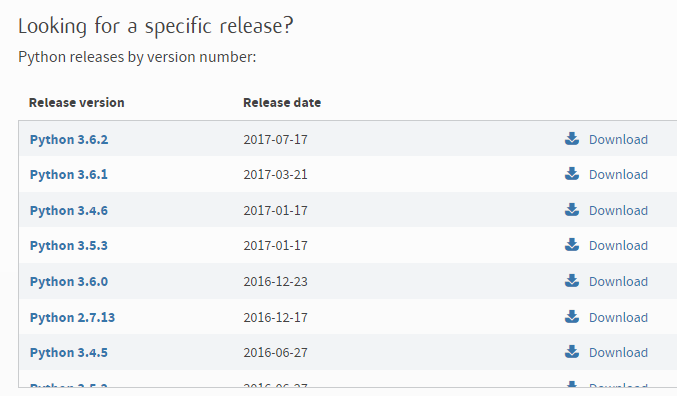
\includegraphics[width=1.0\textwidth]{figs/pythonVer.png}
\end{figure}
\end{frame}

\begin{frame}{Install Python - two choices}
For numerical and scientific work I recommend installing Anaconda or Enthought Canopy. These installations include the most popular libraries that are pre-built for your system. (I prefer Canopy, but use both.)
  \begin{columns}[onlytextwidth]
    \column{0.5\textwidth}
          \begin{figure} 	
 	
\includegraphics[width=1.0\textwidth]{figs/anaconda_logo.png}

      \end{figure}
    \column{0.5\textwidth}
          \begin{figure} 	
 	
\includegraphics[width=1.0\textwidth]{figs/canopy-logo.png}

      \end{figure}
  \end{columns}
  
 Only a few months ago did Canopy start support Python~3.X, while Anaconda has supported Python~3.X for some time. I don't like Spyder IDE included with Anaconda because you can't bind crt + / to comment..
\end{frame}

\begin{frame}{Install Anaconda if ...}
You want
\begin{itemize}
\item to have it your way
\item to run multiple Python versions
\item install TensorFlow or other ML libraries on Windows
\item the powerful conda console tool for installing libraries
\item the latest and greatest Python libraries
\item Spyder IDE
\item automatic environmental variable setup
\end{itemize}

\end{frame}

\begin{frame}{Install Enthought Canopy if ...}
You want
\begin{itemize}
\item the easiest Python scientific environment
\item a pretty GUI for library management and updates
\item Canopy IDE
\item fewer options
\end{itemize}

\end{frame}

\begin{frame}{If you are coming from MATLAB ...}
\textbf{Useful resources}
\url{http://mathesaurus.sourceforge.net/matlab-numpy.html}
\url{https://docs.scipy.org/doc/numpy-dev/user/numpy-for-matlab-users.html}
\end{frame}

\begin{frame}{Install Python - Anaconda}
Anaconda gives you more control over which Python version. Also Anaconda updates more frequently.
\url{https://www.continuum.io/downloads}
          \begin{figure} 	
 	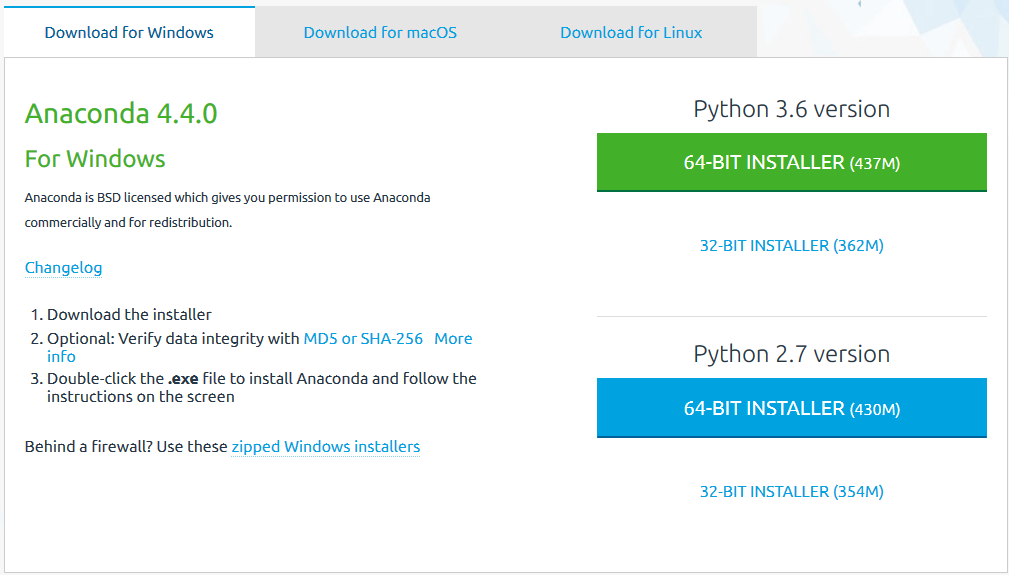
\includegraphics[width=1.0\textwidth]{figs/anaconda.png}
      \end{figure}
\end{frame}

\begin{frame}{GOLDEN RULE with software...}
	\begin{alertblock}{my golden rule}
If you don't know what advanced options do in software (especially when installing new software), leave the advanced options to their default setting. This will come up during the Anaconda installation.
	\end{alertblock}
\end{frame}

\begin{frame}{Anaconda - Advanced Options}
Checking the top box will add the Anaconda installation to your PATH environment variable. Do this on Windows if you want access to python, ipython, pip, and conda from any command prompt or shell on your system for your user. If you don't check the top box, you can always access these applications from the \textit{Anaconda Prompt}.

\begin{figure}
 	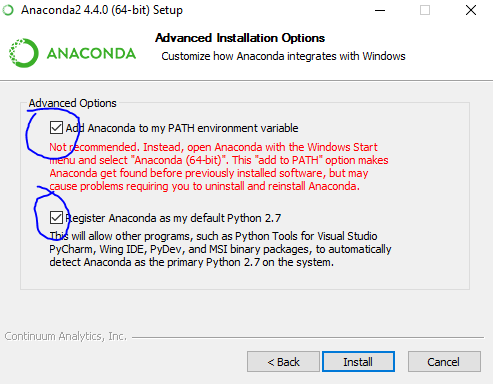
\includegraphics[width=0.5\textwidth]{pythonInstall/anacondaCheck.png}
\end{figure}

\textbf{On Linux} (and maybe macOS) do not check the top box.
\end{frame}

\begin{frame}{Spyder IDE installed with Anaconda}
          \begin{figure} 	
 	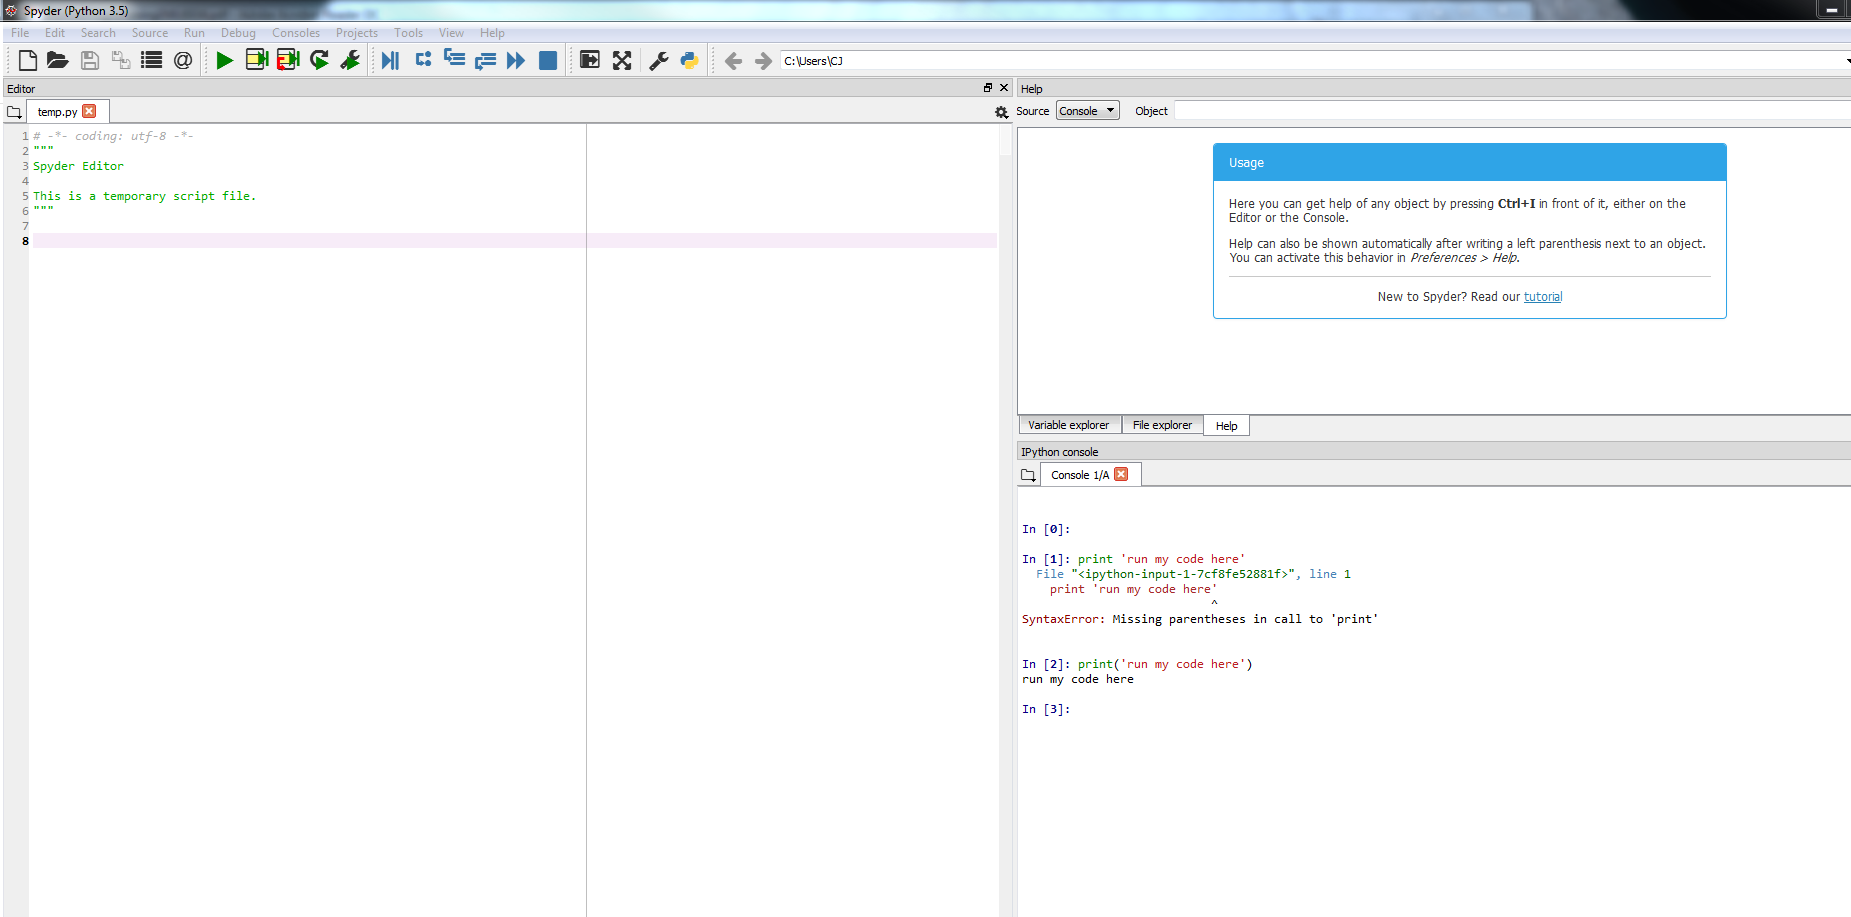
\includegraphics[width=1.0\textwidth]{figs/spyder.png}
      \end{figure}
\end{frame}

\begin{frame}{Install Python - Enthought Canopy}
With Enthought Canopy you may either install Python~2.7 or Python~3.5
\url{https://store.enthought.com/downloads/}
          \begin{figure} 	
 	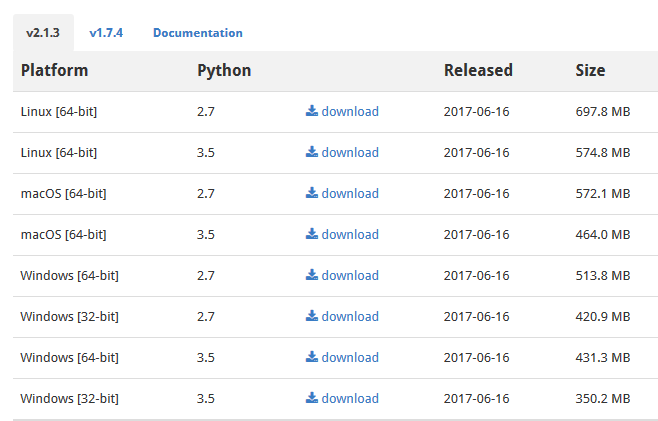
\includegraphics[width=1.0\textwidth]{figs/canopyInstall.png}
      \end{figure}
\end{frame}

\begin{frame}{Canopy no longer sets up your environment variables by default...}
In order to run Python from any command prompt/ shell on your Windows computer, I recommend adding the recently installed python directories to your PATH.

\path{C:\Users\yourUserNameHere\AppData\Local\Enthought\Canopy\edm\envs\User}

\path{C:\Users\yourUserNameHere\AppData\Local\Enthought\Canopy\edm\envs\User\scripts}

On Windows 7, 8, and 10 go to System $>$ Advanced System Settings $>$ environment variables.

In Windows environment variables are separated without spaces using ;

(If you didn't check the boxes with Anaconda, you'll need to set up the environment variables yourself)
\end{frame}

\begin{frame}{Canopy editor IDE installed with Enthought Canopy}
          \begin{figure} 	
 	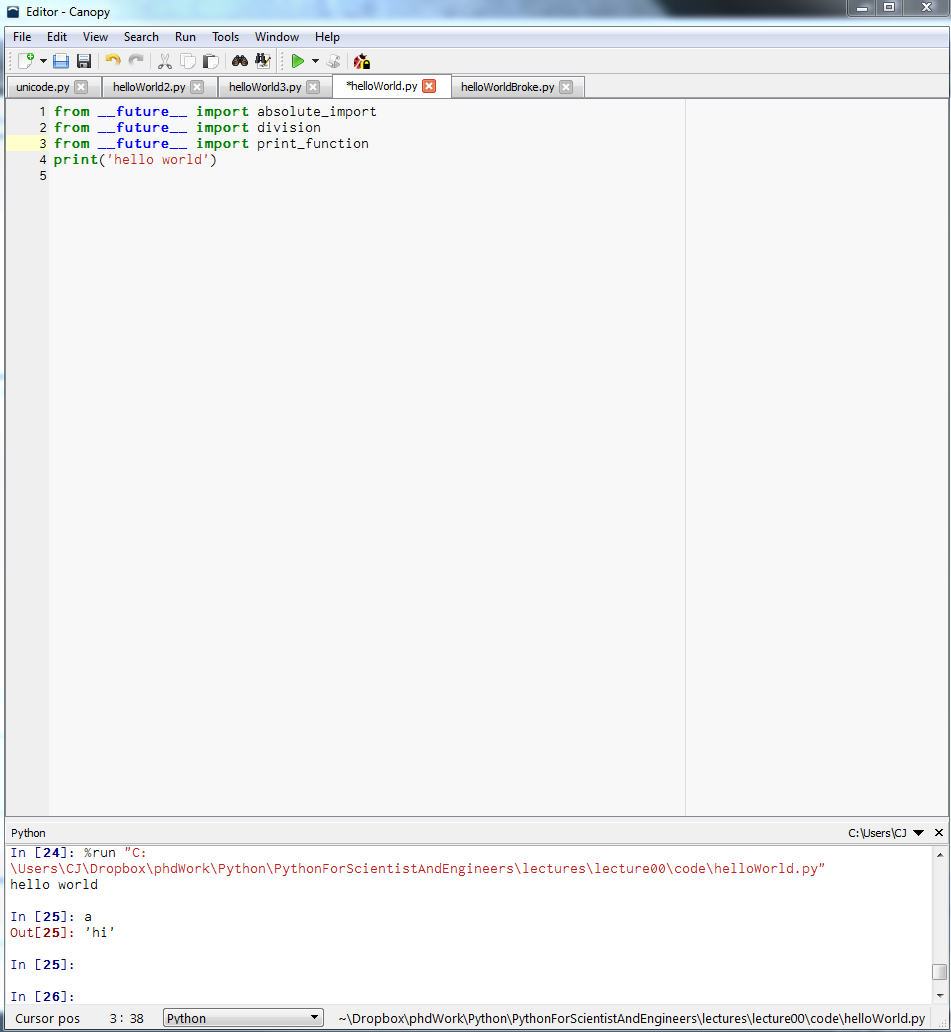
\includegraphics[width=.75\textwidth]{figs/canopy.png}
      \end{figure}
\end{frame}


\begin{frame}{Anaconda vs Enthought Canopy doesn't matter for this course}
... but what does matter is that you have a working Python installation with pre-built scientific libraries.
\end{frame}

\begin{frame}{If you added Python to your PATH - Make sure it works}
You can run python from the command line by typing python in your favorite shell/command prompt.

\begin{figure}
 	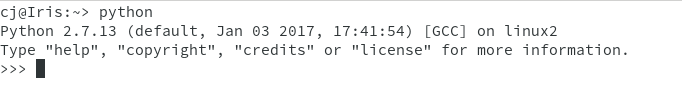
\includegraphics[width=1.0\textwidth]{figs/pythonLinux.png}
\end{figure}

On Windows (Open up a command prompt and type python followed by an enter). To open up a command prompt, hit the windows key and type command prompt. You should see a command prompt show up in the search.

\end{frame}

\begin{frame}{If you did not add Python to your PATH}
Open up the Anaconda Prompt, and type python followed by an enter to open the python interpreter to make sure it is working.

If you installed Enthought Canopy, open up the editor. Then go to tools on the top ribbon $>$ and open Canopy Prompt. When the command prompt opens type python hit enter. 

To exit the Python interpreter, type exit() followed by an enter.
\end{frame}

%\begin{frame}{Also make sure that you can run pip }
%Also please ensure that you can run pip from your favorite shell/command prompt. 
%
%\begin{figure}
% 	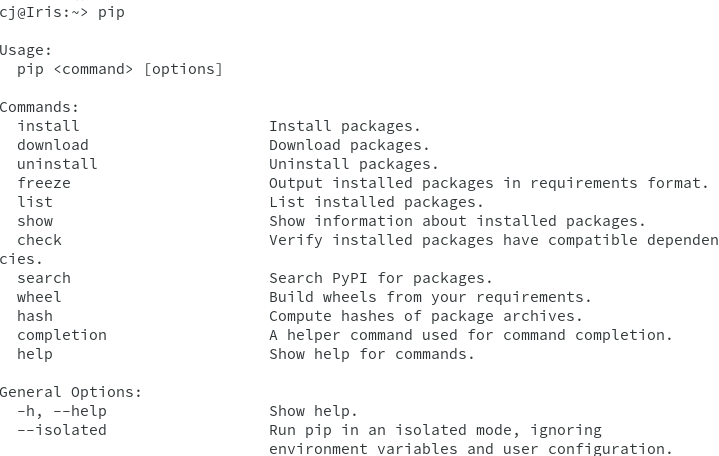
\includegraphics[width=1.0\textwidth]{figs/pipLinux.png}
%
%\end{figure}
%
%\end{frame}

\begin{frame}{HW 00: due one week from today - turn in online before class starts}
This HW will appear as a Quiz in Canvas. If you don't see the canvas Quiz please let me know!
\begin{enumerate}
\item Install Python. A) Tell me if you installed Anaconda or Enthought Canopy. B) Tell me which python version you installed (2.7, 3.5, 3.6?).
\item What operating system do you use? (Ex: Windows 7, OS X Yosemite, Ubuntu 14)
\item What previous programming languages are you familiar with? (Hint: only name the ones you have used the most)
\end{enumerate}
\end{frame}

\begin{frame}{Tools used to make this presentation}
This presentation was made with Beamer using \LaTeX. Texmaker is my favorite cross-platform \LaTeX ~editor. I use Metropolis, a modern Beamer theme. Syntax highlighting is done using Minted and Pygmentex. I use pdfpc (PDF presenter console) to present PDF files. 

Links:
\begin{itemize}
\item \url{https://en.wikipedia.org/wiki/Beamer\_(LaTeX)}
\item \url{https://www.latex-project.org/}
\item \url{http://www.xm1math.net/texmaker/}
\item \url{https://github.com/matze/mtheme}
\item \url{https://www.ctan.org/pkg/minted?lang=en}
\item \url{https://www.ctan.org/pkg/pygmentex?lang=en}
\item \url{https://pdfpc.github.io/}
\end{itemize} 

\end{frame}



%\begin{frame}{Table of contents}
%  \setbeamertemplate{section in toc}[sections numbered]
%  \tableofcontents[hideallsubsections]
%\end{frame}

%\section{About Me}

%\begin{frame}{Introduction}
%\textbf{EML4930/EML6934} | Python Programming | R4 
%
%	The course on Python will cover
%	\begin{itemize}
%	\item The basics (loops, lists, objects, etc.)
%	\item Matrix operations and linear algebra
%	\item Plotting
%	\item Statics (distributions, regression, DOE)
%	\item Optimization algorithms
%	\item Libraries: NumPy, SciPy, Matplotlib, scikit-learn
%	\end{itemize}
%\end{frame}
%
%\begin{frame}{Outline for this talk}
%\begin{enumerate}
%\item About the course
%\item About Me
%\item What is Python? 
%\item Why Python?
%\end{enumerate}
%\end{frame}
%
%\begin{frame}{About the course: Course description}
%	\begin{alertblock}{Course description}
%Python is a general purpose programming language. Course covers the basics, linear algebra, plotting, and more to prepare students for solving numerical problems. Prerequisite: COP 2271 MATLAB or equivalent.
%	\end{alertblock}
%	
%	
%	
%	I believe I'm more productive with Python. I'd like to help others learn Python.
%\end{frame}
%
%\begin{frame}{About the course: Tentative lecture outline}
%\begin{enumerate}
%\item About Python (2 vs 3), IDEs, iPython, notebooks, and installation
%\item Basics: data types, math, loops 
%\item Python classes, objects, namespace
%\item Python libraries and pip
%\item Numpy and Matrix operations
%\item More Numpy and Matplotlib for 2D plots
%\item Contour plots, 3D plot, Histograms
%\item Statistical distributions and functions
%\item Optimization in Scipy
%\item Python read and write: opening and modifying text/csv files
%\item Symbolic math with SymPy, DOE with pyDOE
%\item Scikit-learn: surrogate modeling 
%\item Scikit-learn: surrogate modeling and machine learning
%\item Pandas and DataFrames
%\end{enumerate}
%\end{frame}
%
%\begin{frame}{About me: Background with Python}
%I use Python to do everything.
%
%In 2014 I switched from MATLAB to Python, and have never looked back.
%
%My first Python project involved plotting the results for a non-linear FE routine.
%
%Python allows me implement new ideas faster than other languages.
%
%There are Python libraries to do \textit{just about} everything. 
%\end{frame}
%
%\begin{frame}{About me: Python projects}
%Things I've created in Python:
%\begin{itemize}
%\item FE cylindrical mesher
%\item HPC optimization managing
%\item Various FE optimization
%\item Power outage twitter bot
%\item Piecewise linear fit library
%\item Roulette game
%\item and more!
%\end{itemize}
%\end{frame}
%
%\begin{frame}{What is Python? - import antigravity}
%      	\begin{figure} 	
% 	\includegraphics[width=0.65\textwidth]{images/python.png}
%      \end{figure}
%\end{frame}
%
%\begin{frame}{What is Python? - python.org}
%Let's see what \url{http://python.org} has to say about Python.
%      	
%      	\begin{figure} 	
% 	
\includegraphics[width=0.65\textwidth]{images/pythonLogo.png}
%      \end{figure}
%
%\textbf{Python is}
%\begin{itemize}
%\item an interpreted, object-oriented, high-level programming language with dynamic semantics
%\item very attractive for Rapid Application Development
%\item a simple and easy to learn syntax
%\end{itemize}
%\end{frame}
%
%\begin{frame}{What is Python? - A toolbox for engineers }
%
%\textbf{Python is}
%\begin{itemize}
%\item \textbf{free} and \textbf{open source}
%\item viable replacement of MATLAB for everyday use
%\item for numerical and scientific research
%\item great for working for data
%\end{itemize}
%      	\begin{figure} 	
% 	\includegraphics[width=0.5\textwidth]{images/pythondata.jpg}
%      \end{figure}
%\end{frame}
%
%\begin{frame}{What is Python? - famous applications built with Python}
%\begin{figure}
%\includegraphics[width=1.0\textwidth]{images/logos.png}
%\end{figure}
%%      	\begin{figure} 	
%% 	\includegraphics[width=0.33\textwidth]{images/youtube.png}
%% 	 	\includegraphics[width=0.33\textwidth]{images/googlelogo.png}
%% 	\includegraphics[width=0.33\textwidth]{images/dropboxlogo.png}
%%      \end{figure}
%%          \begin{figure} 	
%% 	\includegraphics[width=0.33\textwidth]{images/quora.png}
%% 	 	\includegraphics[width=0.33\textwidth]{images/instgram.jpg}
%% 	 	\includegraphics[width=0.33\textwidth]{images/bittorrent.png}
%%      \end{figure}
%%          \begin{figure} 	
%% 	\includegraphics[width=0.33\textwidth]{images/spotify.png}
%% 	\includegraphics[width=0.33\textwidth]{images/reddit.png}
%% 	\includegraphics[width=0.33\textwidth]{images/yahoomaps.png}
%%
%%      \end{figure}
%\end{frame}
%
%
%\begin{frame}{Why Python? - beautiful and simple syntax}
%You may not know Python, but intuitively you already understand the following Python code.
%    \inputminted{python}{code/readlines.py}
%
%\end{frame}
%
%\begin{frame}{Why Python? - Surrogate modeling library scikit-learn 1/2}
%  \begin{columns}[onlytextwidth]
%    \column{0.7\textwidth}
%    scikit-learn - machine learning in Python    
%	\textbf{Regression}
%	\begin{itemize}
%	\item Ordinary least squares
%	\item Bayesian regression
%	\item Kernel ridge regression
%	\item Support vector regression
%	\item Stochastic gradient regression
%	\item Nearest neighbors regression
%	\item Gaussian process regression (Kriging)
%	\item Decision tree regression
%	\item Gradient tree boosted regression
%	\item Neural network regression
%	\item \textbf{And MORE!}
%	\end{itemize}
%    \column{0.3\textwidth}
%          \begin{figure} 	
% 	\includegraphics[width=1.0\textwidth]{images/sklearn.png}
%
%      \end{figure}
%  \end{columns}
%\end{frame}
%
%\begin{frame}{Why Python? - Surrogate modeling library scikit-learn 2/2}
%  \begin{columns}[onlytextwidth]
%    \column{0.7\textwidth}
%    
%    scikit-learn - machine learning in Python    
%	\textbf{Dimensional reduction}	
%	\begin{itemize}
%	\item PCA
%	\item LDA
%	\end{itemize}
%	\textbf{Reprocessing}
%	\begin{itemize}
%	\item Unit variance scaling
%	\item Scaling with outliers
%	\item Normalization
%	\item \textbf{and MORE!}
%	\end{itemize}
%	\textbf{Model selection}
%	\begin{itemize}
%	\item Cross validation
%	\item Parameter tuning methods
%	\item Model scoring metrics
%	\item \textbf{and MORE!}
%	\end{itemize}
%    \column{0.3\textwidth}
%          \begin{figure} 	
% 	\includegraphics[width=1.0\textwidth]{images/sklearn.png}
%
%      \end{figure}
%  \end{columns}
%\end{frame}
%
%\begin{frame}{Why Python? - beautiful documentation 1/4}
%          \begin{figure} 	
% 	\includegraphics[width=1.0\textwidth]{images/sklearnWeb.png}
%
%      \end{figure}
%\end{frame}
%
%\begin{frame}{Why Python? - beautiful documentation 2/4}
%          \begin{figure} 	
% 	\includegraphics[width=1.0\textwidth]{images/sklearnSVR.png}
%
%      \end{figure}
%\end{frame}
%
%\begin{frame}{Why Python? - beautiful documentation 3/4}
%          \begin{figure} 	
% 	\includegraphics[width=1.0\textwidth]{images/sklearnSVR1.png}
%
%      \end{figure}
%\end{frame}
%
%\begin{frame}{Why Python? - beautiful documentation 4/4}
%          \begin{figure} 	
%          \caption{SVR example from \url{http://scikit-learn.org/stable/auto_examples/svm/plot_svm_regression.html}}
% 	\includegraphics[width=.85\textwidth]{images/sklearnSVR2.png}
%
%      \end{figure}
%\end{frame}
%
%\begin{frame}{Why Python? - the latest and greatest in Machine learning}
%TensorFlow and theano are the best machine learning libraries complete with the latest in deep learning techniques. 
%  \begin{columns}[onlytextwidth]
%    \column{0.5\textwidth}
%          \begin{figure} 	
% 	
\includegraphics[width=1.0\textwidth]{images/tf.png}
%
%      \end{figure}
%    \column{0.5\textwidth}
%          \begin{figure} 	
% 	\includegraphics[width=1.0\textwidth]{images/theano.jpg}
%
%      \end{figure}
%  \end{columns}
%\end{frame}
%
%\begin{frame}{Why Python? - Python is already installed on OSX and Linux}
%
%  \begin{columns}[onlytextwidth]
%    \column{0.5\textwidth}
%          \begin{figure} 	
% 	\includegraphics[width=1.0\textwidth]{images/OS-X-Yosemite-Logo.jpg}
%
%      \end{figure}
%    \column{0.5\textwidth}
%          \begin{figure} 	
% 	\includegraphics[width=1.0\textwidth]{images/linux.png}
%
%      \end{figure}
%  \end{columns}
%\end{frame}
%
%\begin{frame}{Why Python? - Python works great on Windows too!}
%          \begin{figure} 	
% 	\includegraphics[width=1.0\textwidth]{images/pythonWindows.png}
%      \end{figure}
%\end{frame}
%
%\begin{frame}{Why Python? - Free, Open, and Powerful}
%
%
%  \begin{columns}[onlytextwidth]
%    \column{0.7\textwidth}
%    
%\begin{itemize}
%\item Python is Free and Open
%\item Python can be used commercially 
%\item From research to deployment
%\item Libraries to do everything
%\item Cross platform support
%\end{itemize}
%    \column{0.3\textwidth}
%          \begin{figure} 	
% 	
\includegraphics[width=1.0\textwidth]{images/free-beer.jpg}
%
%      \end{figure}
%  \end{columns}
%
%
%\end{frame}
%
%\begin{frame}{Why Python? - 2014 IEEE Spectrum}
%
%\begin{figure}
%\caption{In 2014 IEEE Spectrum rated MATLAB as 10th most popular language, while Python was the fourth most popular language. \url{http://spectrum.ieee.org/static/interactive-the-top-programming-languages}}
% 	\includegraphics[width=0.8\textwidth]{images/2014.png}
% 
%\end{figure}
%
%\end{frame}
%
%\begin{frame}{Why Python? - 2016 IEEE Spectrum}
%
%\begin{figure}
%\caption{In 2016 IEEE Spectrum rated MATLAB as 12th most popular language, while Python was the third most popular language. \url{http://spectrum.ieee.org/static/interactive-the-top-programming-languages-2016}}
% 	\includegraphics[width=0.8\textwidth]{images/2016.png}
% 
%\end{figure}
%
%\end{frame}
%
%\begin{frame}{Conclusion}
%\textbf{EML4930/EML6934 | Python Programming | 1 credit
%}
%
%MATLAB is becoming less popular for scientist and engineers while Python is growing fast. 
%
%How long can \textbf{you} be competitive without knowing Python? 
%
%I'm open to suggestions on course specifics. Let me know if there is something specific you'd like covered.
%\end{frame}
%

%
%\begin{frame}{Matlab vs Python: code comparison}
%\textbf{Python}:
%    \inputminted{python}{code/code.py}
%\textbf{MATLAB}:
%    \inputminted{matlab}{code/code.m}
% 
%%\lstinputlisting[language=Python,caption=Python example]{code/code.py}
%\end{frame}
%
%\begin{frame}{Let's take a look at what Mathworks has to say about Python}
%          \begin{figure} 	
% 	\includegraphics[width=1.0\textwidth]{images/matlablies.png}
%      \end{figure}
%	\begin{alertblock}{Disclaimer}
%	I'm teaching a course in Python and use Python for everything. My views on MATLAB will contain bias.
%	\end{alertblock}
%\end{frame}
%
%\begin{frame}{MATLAB vs Python: what Mathworks has to say}
%The difference is clear: MATLAB is the easiest and most productive computing environment for engineers and scientists. It includes the MATLAB language, the only top programming language dedicated to mathematical and technical computing.
%
%In contrast, Python is a general-purpose programming language requiring add-on libraries for performing even basic mathematics.
%
%\url{http://mathworks.com/products/matlab/matlab-vs-python.html}
%\end{frame}
%
%\begin{frame}{MATLAB vs Python: from my perspective}
%The difference is clear: Python is the easiest programming language. Python is complete with the latest library developments created by scientist and engineers. Python is the best free and open alternative to MATLAB.
%
%In contrast, MATLAB is a very expensive linear algebra solver with great solutions for control systems.
%
%\end{frame}


%\begin{frame}{MATLAB vs Python: Mathworks speed comparison}
%  \begin{columns}[onlytextwidth]
%    \column{0.3\textwidth}
%      \begin{itemize}
%        \item There is no basis for these findings \item If you care about speed, MATLAB is the wrong language! \item Use the money saved on faster hardware \item Python performance per cost is infinity times better
%      \end{itemize}	
%    \column{0.7\textwidth}
%          \begin{figure} 	
% 	\includegraphics[width=.85\textwidth]{images/matlabFaster.jpg}
%
%      \end{figure}
%  \end{columns}
%
%\url{http://mathworks.com/products/matlab/matlab-vs-python.html}
%\end{frame}
%\begin{frame}{My research}
%\begin{itemize}
%	\item Structural optimization
%	\item Non-linear finite element (FE) analysis
%	\item Non-linear regression
%	\item Material parameter identification
%\end{itemize}
%\end{frame}
%
%\begin{frame}{Identifying material parameters for FEA}
%\begin{itemize}
%	\item There are lots of different material models
%	\item Various non-linear behavior
%	\item Often no physical link between model parameters and experiment
%	\item But we have experimental data from some physical test
%\end{itemize}
%     \metroset{block=fill}
%      \begin{block}{Goal: Find the best set of material parameters such that}
%          the FE model produces a response analogous to the experimental data
%      \end{block}
%      	\begin{figure} 	
% 	\includegraphics[width=0.45\textwidth]{images/Weichert.pdf}
%      \end{figure}
%\end{frame}
%
%\begin{frame}{Why is this important?}
%\begin{itemize}
%	\item Structural FE models are only as good as the material model!
%	\item If our FE model can't replicate the material behavior - 
%	\item Will the FE model be able replicate the structural behavior? 
%\end{itemize}
%	\begin{figure} 	
% 	\includegraphics[width=1.0\textwidth]{images/garbage.jpg}
%      \end{figure}
%      Fair use figure taken from  https://www.linkedin.com/
%\end{frame}
%
%\begin{frame}{PVC-coated polyester}
%  \begin{columns}[onlytextwidth]
%    \column{0.4\textwidth}
%      \begin{itemize}
%        \item highly non-linear \item plain orthogonal weave  \item often assumed linear orthotropic \item Find non-linear orthotropic parameters
%      \end{itemize}	
%    \column{0.6\textwidth}
%	\begin{figure} 	
% 	\includegraphics[width=1.0\textwidth]{images/900gsm-pvc-coated-polyester-width-300cm-1-1.jpg}
%      \end{figure}
%  \end{columns}
%\end{frame}
%
%\begin{frame}{Uniaxial tests in warp - fill - $45^\circ$~bias material directions}
%Uniaxial tests performed in three distinct fiber directions. Digital image correlation (DIC) used to provide the full displacement field of the uniaxial test. 
%  \begin{columns}[onlytextwidth]
%    \column{0.5\textwidth}
%	\begin{figure} 	
% 		\includegraphics[width=1.0\textwidth]{images/44_criterion.jpg}
%    \end{figure}
%    \column{0.5\textwidth}
%	\begin{figure} 	
% 		\includegraphics[width=1.0\textwidth]{images/strainMasterPortable.jpg}
%    \end{figure}
%  \end{columns}
%\end{frame}
%
%\begin{frame}{Experimental data}
%	\begin{figure}
%	\caption{Experimental data collected from Uniaxial tests in the warp, fill, and $45^\circ$~bias fiber directions. Noise is seen in the data from repeating each test direction five times.} 	
% 		\includegraphics[width=0.75\textwidth]{images/noNoise.pdf}
%    \end{figure}
%\end{frame}
%
%\begin{frame}{3 finite element models - one for each material direction}
%\begin{itemize}
%\item FE models created in MSC Marc
%\item One model for each test direction
%\item Models replicate uniaxial test
%\item Non-linear FEA
%\end{itemize}
%	\begin{figure} 	
% 		\includegraphics[width=1.0\textwidth]{images/45bias.jpg}
%    \end{figure}
%\end{frame}
%
%\begin{frame}{Non-linear orthotropic material model}
%The non-linear orthotropic model is defined below, where stiffness moduli are functions of strain. 
%\begin{equation}
%E_1(\varepsilon_1) = \beta_0 + \beta_1\varepsilon_1 + \beta_2\varepsilon_1^2 + \beta_3\varepsilon_1^3
%\end{equation}
%\begin{equation}
%E_2(\varepsilon_2) = \beta_4 + \beta_5\varepsilon_2 + \beta_6\varepsilon_2^2
%\end{equation}
%\begin{equation}
%G_{12}(\gamma_{12}) = \beta_7 + \beta_8\gamma_{12} + \beta_9\gamma_{12}^2
%\end{equation}
%
%Use optimization to find the best set of $\bm{\beta}$ parameters to minimize error between FE models and data.
%\end{frame}
%
%\begin{frame}{Non-linear regression - root mean square error}
%Root mean square (RMS) error is calculated for each test direction.
%\begin{equation}\label{eq:eWarp}
%e_\text{warp} = \sqrt{\frac{\sum_i^n [F_\text{warp}(x_i) - P_\text{warp}(x_i)]^2 }{n}}
%\end{equation}
%
%\begin{equation}
%e_\text{fill} = \sqrt{\frac{\sum_i^n [F_\text{fill}(x_i) - P_\text{fill}(x_i)]^2 }{n}}
%\end{equation}
%
%\begin{equation}\label{eq:eBias}
%e_\text{bias} = \sqrt{\frac{\sum_i^n [F_\text{bias}(x_i) - P_\text{bias}(x_i)]^2 }{n}}
%\end{equation}
%
%The RMS errors are combined into a single error value $e_u$.
%\begin{equation}\label{eq:eUniaxial}
%e_u = \sqrt{e^2_\text{warp} + e^2_\text{fill} + e^2_\text{bias}}
%\end{equation}
%
%\end{frame}
%
%\begin{frame}{Using optimization to minimize RMSE}
%Find the optimum set of $\bm{\beta}^\star$ that
%\begin{equation}
%\label{eqn:optimzeGoalUni}
%\begin{split}
%\textrm{minimize:} & \quad e_{u}\\
%\textrm{such that:} & \quad E_1, E_2, G_{12} > 0 \quad \textrm{and}\\
%& \textrm{All Marc Exit Codes} = 3004
%\end{split}
%\end{equation}
%Constrained optimization problem, solved using the gradient based MMFD from multiple starting points $\bm{\beta_0}$.
%\end{frame}
%
%\begin{frame}{The resulting $\bm{\beta}^\star$ material model}
%	\begin{figure}
%	\caption{The material model found through non-linear regression produces FE models that match the experimental uniaxial response. } 	
% 		\includegraphics[width=1.0\textwidth]{images/plotStrainGageDataWithMatBlack.pdf}
%    \end{figure}
%\end{frame}
%
%\begin{frame}{Calculation of standard errors}
%Linearization is performed according to \cite{Coppe2011}, in order to calculate the standard errors. Use local approximations to construct a linear regression matrix $\bm{X}$.
%\begin{equation}\label{eq:regMatrixX}
%\bm{X} = \begin{bmatrix}
%\frac{\partial f_u(x_1, \bm{\beta}^\star)}{\partial \beta_1} & \frac{\partial f_u(x_1, \bm{\beta}^\star)}{\partial \beta_2} & \dots & \frac{\partial f_u(x_1, \bm{\beta}^\star)}{\partial \beta_{n_\beta}} \\
%\frac{\partial f_u(x_2, \bm{\beta}^\star)}{\partial \beta_1} & \frac{\partial f_u(x_2, \bm{\beta}^\star)}{\partial \beta_2} & \dots & \frac{\partial f_u(x_2, \bm{\beta}^\star)}{\partial \beta_{n_\beta}} \\
%\vdots & \vdots & \ddots & \vdots \\
%\frac{\partial f_u(x_n, \bm{\beta}^\star)}{\partial \beta_1} & \frac{\partial f_u(x_n, \bm{\beta}^\star)}{\partial \beta_2} & \dots & \frac{\partial f_u(x_n, \bm{\beta}^\star)}{\partial \beta_{n_\beta}} \\
%\end{bmatrix}
%\end{equation}
%\begin{equation}\label{eq:SE}
%\text{SE}(\beta_j) = \hat{\sigma} \sqrt{[\bm{X}^\text{T}\bm{X}]^{-1}_{jj}}, \quad \quad j = 1, 2, \dots, n_\beta 
%\end{equation}
%\end{frame}
%
%\begin{frame}{Standard errors into confidence interval}
%\begin{table}[hbt!]
%\centering
%% table caption is above the table
%\caption{Standard errors allows us to find the confidence interval on the non-linear regression results. Table shows 95\% confidence interval bounds on the optimal values determined from the optimization.}
%\label{tab:black95bounds}       % Give a unique label
%% For LaTeX tables use
%\begin{tabular}{lccc}
%\noalign{\smallskip}
%Variable & 95\% LB & Value & 95\% UB \\
%\noalign{\smallskip}\hline\noalign{\smallskip}
%$\beta_0$ & 0.975 & 1.001  & 1.028 \\
%$\beta_1$ & -27.0 & -25.9  & -24.7 \\ 
%$\beta_2$ & 284.3 & 293.6  & 302.9 \\
%$\beta_3$ & -865. & -845.  & -825. \\
%$\beta_4$ & 0.324 & 0.346  & 0.367 \\
%$\beta_5$ & -5.20 & -4.47  & -3.74 \\
%$\beta_6$ & 26.18 & 30.68  & 35.18 \\
%$\beta_7$ & 0.028 & 0.033  & 0.038 \\
%$\beta_8$ & -0.33 & -0.29  & -0.24 \\
%$\beta_9$ & 0.811 & 0.891  & 0.971 \\
%\hline
%\end{tabular}
%\end{table}
%\end{frame}
%
%\begin{frame}{Conclusions}
%	\begin{itemize}
%	\item Computational expensive non-linear FE models
%	\item Time consuming setup - problem specific
%	\item Hidden dangers of this approach
%	\item This approach is commonly called an inverse analysis
%	\item Practical example of structural optimization and non-linear regression
%	\item For more information on this specific problem see:  \cite{Jekel2016a} and \cite{Jekel2017a}
%	\end{itemize}
%\end{frame}
%
%\begin{frame}[allowframebreaks]{References}
%
%  \bibliography{phdThesis}
%  \bibliographystyle{abbrv}
%
%\end{frame}

\end{document}
